\documentclass[reqno,12pt,oneside]{report}
\usepackage[utf8]{inputenc}
\usepackage{extra/rac} 
\usepackage[intlimits]{amsmath}
\usepackage{amsxtra}
\usepackage{amsthm}
\usepackage{amssymb}
\usepackage{graphicx} 
\usepackage{rotating}
\usepackage{color}
\usepackage{xspace}
\usepackage{mdframed}
\usepackage{epsfig}
\usepackage{subfigure} 
\usepackage{multirow}
\usepackage{verbatim}
\usepackage[numbers]{natbib}     
\usepackage{acronym}
\usepackage{booktabs}
\usepackage{indentfirst}
\usepackage{enumitem}
\usepackage{setspace}
\usepackage{algpseudocode}
\usepackage{ifthen}
\usepackage[intoc]{nomencl}
\usepackage{tikz}
\usepackage{url}
\usepackage[breaklinks]{hyperref}
\usepackage{hyperref}
\usepackage{algorithm,algpseudocode}
\usepackage[nottoc,notlof,notlot]{tocbibind}
\usepackage{algorithm}
\DeclareUnicodeCharacter{03B2}{\ensuremath{\beta}}
\DeclareUnicodeCharacter{2212}{-}
\newcommand{\tabitem}{~~\llap{\textbullet}~~}
\usetikzlibrary{shapes.geometric, arrows}
\tikzstyle{startstop} = [rectangle, rounded corners, minimum width=3cm, minimum height=1cm,text centered, draw=black, fill=red!30]
\tikzstyle{io} = [trapezium, trapezium left angle=70, trapezium right angle=110, minimum width=3cm, minimum height=1cm, text centered, draw=black, fill=blue!30]
\tikzstyle{process} = [rectangle, minimum width=3cm, minimum height=1cm, text centered, draw=black, fill=orange!30]
\tikzstyle{decision} = [diamond, minimum width=3cm, minimum height=1cm, text centered, draw=black, fill=green!30]
\tikzstyle{arrow} = [thick,->,>=stealth]
\renewcommand\bibname{References}
\makenomenclature
\onehalfspacing 
\newcommand{\sun}{\ensuremath{\odot}}
\theoremstyle{plain}
\newtheorem{theorem}{Theorem}
\newtheorem{prop}[theorem]{Proposition}
\newtheorem{corollary}[theorem]{Corollary}
\newtheorem{lemma}[theorem]{Lemma}
\newtheorem{question}[theorem]{Question}
\newtheorem{conjecture}[theorem]{Conjecture}
\newtheorem{assumption}[theorem]{Assumption}
\theoremstyle{definition}
\newtheorem{definition}[theorem]{Definition}
\newtheorem{notation}[theorem]{Notation}
\newtheorem{condition}[theorem]{Condition}
\newtheorem{example}[theorem]{Example}
\newtheorem{introduction}[theorem]{Introduction}
\theoremstyle{remark}
\newtheorem{remark}[theorem]{Remark}
\numberwithin{theorem}{chapter}  
\makeatletter
\def\cleardoublepage{\clearpage\if@twoside \ifodd\c@page\else
\hbox{}
\thispagestyle{empty}
\newpage
\if@twocolumn\hbox{}\newpage\fi\fi\fi}
\makeatother
\newcommand{\todo}[1]{\vspace{5 mm}\par \noindent
\marginpar{\textsc{To Do}}
\framebox{\begin{minipage}[c]{0.95 \textwidth}
\tt\begin{center} #1 \end{center}\end{minipage}}\vspace{5mm}\par}



\begin{document}

% Title page as required by Rackham dissertation guidelines
\titlepage{Stock Market Analysis Using Twitter Sentiment}{\\Md. Soliman Hossain (172485)\\Munira Ferdous (172514)\\Adiba Masud (172472)}{Bachelor of Science in Information Technolog}
{Information Technology}{March, 2022}{Manan Binth Taj Noor, \\Assistant Professor}

% Begin the front matter as required by Rackham dissertation guidelines
\initializefrontsections
\makeatletter
\if@twoside \setcounter{page}{4} \else \setcounter{page}{1} \fi
\makeatother

%Optional declaration page
\startdeclarationpage
We hereby declare that this thesis is based on the results found by ourselves.
Materials of work found by other researcher are mentioned by reference. This thesis,
neither in whole nor in part, has been previously submitted for any degree.

\vspace{1in}


\noindent \begin{tabular}{p{4cm}p{.5cm}p{4cm}p{.5cm}p{4cm}}
\centering        
    % \includegraphics[scale=0.2]{sig/adiba.png}&& 
    % \includegraphics[scale=0.3]{sig/soliman.png}&& 
    % \includegraphics[scale=0.3]{sig/munira.png}\\
  \rule{4cm}{1pt} && \rule{4cm}{1pt} && \rule{4cm}{1pt}\\
  Md. Soliman Hossain
  &&Adiba Masud
  &&Munira Ferdous \\
  Roll:172485 &&Roll:172472 &&Roll:172514 
\end{tabular}



\label{declaration}

%Optional Certificate page
\startcertificatepage
This is to certify that the thesis entitled \textbf{Stock Market Analysis Using Twitter Sentiment} has been prepared and submitted by \textbf{Munira Ferdous, Md. Soliman Hossain} and \textbf{Adiba Masud} in partial fulfilment of the requirement for the degree of
Bachelor of Science (honors) in Information Technology on March, 2022.
\bigskip
\bigskip
\bigskip

\noindent \begin{tabular}{l}
\rule{4cm}{1pt} \\
Manan Binth Taj Noor\\Supervisor
\end{tabular}

\vspace{.3in}
Accepted and approved in partial fulfilment of the requirement for the degree
Bachelor of Science (honors) in Information Technology.
\vspace{.3in}


\noindent \begin{tabular}{p{4.5cm}p{.5cm}p{4.5cm}p{.5cm}p{4.5cm}}
\centering
     && &&   \\
     && &&   \\
  \rule{4.5cm}{1pt} &  & \rule{4.5cm}{1pt} &  & \rule{4.5cm}{1pt}\\
  Prof. Dr. Md. Abu Yousuf &&Dr. Shahidul Islam &&Dr. Rashed Mazumder\\
  Chairman &&Member &&Member\\
     
     && &&   \\
     && &&   \\
  \rule{5cm}{1pt}\\
  Prof. Dr. Md Hasanul Kabir \\
  Member (External) 
\end{tabular}


\label{Certificate}

% % Optional Acknowledgements page
% \startacknowledgementspage
% \input{introduction/Acknowledgements}
% \label{Acknowledgements}

%Optional Abstract page
\startabstractpage
Recently happening the epidemic which have impacted the importance inquiring ability of our daily life styles. Sentiments have clothed to be a huge impact at the motion of the inventory change and pandemic has satisfactory introduced greater steam. This study with the limelight at the recent pandemic is a try to analyze the magnificence accuracy of determined-on algorithms for sentiment evaluation and prediction for the inventory costs. We’ve attempted to take a look at proposed framework for sentiment analysis and prediction for the ideas to discover the correlation among people and forum sentiment. We use twitter records to anticipate public temper and use the anticipated mood and previous days. We have considerably utilized DJIA values for a certain time period and also tweet values for understanding people’s sentiment on which we are looking ahead to the inventory market actions. After this, checking highlights the accurate process or methods or algorithms based mostly on processed outcomes. Then the ones algorithms may be enough to give input for building active prediction systems such we want. \\
\vspace{4pt}
\textbf{Keywords:} Stock Market, Epidemic, Sentiment Analysis, Twitter Data. 

\label{Abstract}

% List of Abbreviation
\listofabbreviations
\section*{
\begin{center}
  LIST OF ABBREVIATIONS
\end{center}
}
\begin{tabular}{p{2.5cm}p{10cm}}

\textbf{API}  & Application Programming Interface\\
\textbf{LR}  & Linear Regression\\
\textbf{LSTM}  & Long Short-term Memory \\
\textbf{DJIA}  & Dow Jones Industrial Average\\
\textbf{NLP}  & Natural Language Processing\\
\textbf{NLTK}  & Natural Language Toolkit\\
\textbf{SOFNN}  & Self-Organizing Fuzzy Neural Networks \\
\end{tabular}

% List of Notatoin
\listofnotations
\section*{
\begin{center}
 LIST OF NOTATIONS
\end{center}
}

\begin{tabular}{p{2.5cm}p{10cm}}
$\beta$   & Define Beta\\
$\epsilon$  & Define Epsilon\\
$\omega$& Define Omega\\
$\theta$   & Define Theta\\
\end{tabular}


\listoffigures   % Required if there is more than one figure
\tableofcontents     % Required
\printnomenclature[1.5cm]

\startthechapters

 \label{chap0:Introduction}
 \chapter{Introduction}
\section{Background}
Almost two and a half trillion stock investors within the world per 2021 recent statistics are contributing to global economics through the exchange. The overall global stock market trading turnover is around \$95 trillion. Particularly, retail investors have made a buy or sell investment decisions depends on the world situation. Within the whole world, there are plenty of taking resolutions for an investment to involve an outsized volume of cash are produced. Spending a lot of time on uncovering funding lucky chances by retail shareholders has become a day-to-day difficulty. On the other hand, other investors are looking for white-collar commercial advisory services, the prices are sky high only for retail shareholders. For this reason, they are not being able to take that service easily as others and have to make all types decision depending on their own market analysis. So, this type of doing own analysis is becoming very tough in this modern time when there are a lot of technological opportunity.\\

Humans are being sophistical in their behavior at some certain events or matters. While not being valued, task based different thinking, choices get biased by psychological feature biases or personal emotions, resulting in gratuitous losses. The analysis of the company’s shares is currently obsessed with most on completely different social media sites. Among different social media sites that has most significant among the economic and share market empire is Twitter. Almost 500 million tweets are sent by active users on a usual. To express their various emotions through these tweets, which are being translated into helpful info. At now, such an improbable quantity of social media knowledge can’t be entirely accumulated by investors only being alone. It is a just about not possible task for them to make it on their own. Therefore, a processed analysis system is vital for investors, because this system can mechanically appraise stock trends victimization such giant amounts of knowledge in our worked database.\cite{bhavya2021stock}\\ 

Without access to quantitative and information-pushed models on people’s sentiment analysis, one apparent technique retail buyers could use to wager the market is through simple signs, as an example, easy regression and exponential shifting average. Again, there are huge up-downs in the world stock market for last years, due to coronavirus and for it's post covid impact. Like an example, the stock market came crashing down suddenly because of sudden attack of coronavirus and also the finance instability. This crash because caused a huge fall down to the market and after two months again tried to enter at the stock markets, which continued through at the end of the same year. Another noticed matter is when in 2019 the leading company was Microsoft, but in the middle of year 2020, Arabian oil company took the leading which was worth around \$1.36 trillion.\\

To get the analysis of the above information and also for closing prediction of stock prices there have been a lot of experiments caused in these recent years. Supervised learning and unsupervised learning classifications of machine learning models are used consequently to predict the stock prices with the most accurate level. Among those several techniques like the Decision Tree method, Support Vector Machine, KNN, Random Forest method, Naive Bayes method, Logistic Regression are vastly used to apply machine learning model for better prediction. Without these techniques, R programming is also used to plot the data of analyzing and also future prediction.\\

Again, retail investors will be able to predict the stock exchange by drawing a regression line that connects the utmost or minimum of possible prices. A regression system is used to guess and predict the current market trend which is inspired by the adding modern machine learning algorithms for research, these algorithms might serve as implicit tools to seek out actual patterns within the trend of stock prices, this information may be useful to supply redundant perceptivity for retail investors when making different investment planning.\\

Twitter sentiment analysis is an imperial of data and can hand over intuition that can intimate positive or negative discern on stocks and direction. There has an enough number of research on sentiment analysis on different topics, just for movie reviews and Twitter post in random or defined days, months. In this work we use sentiment analysis on twitter random posts. Saving Twitter Sentiment Analysis for implementation by applying twitter API kept by twitter. This method is extirpating tweets from twitter in given below :\\

\begin{itemize}
    \item Firstly, import essential packages and libraries.
    \item Determine criterion which build up relationship with twitter API. 
    \item By removing some words for cleaning the tweets.
    \item Tokenize every phrase withinside the dataset and keep it into the dataset
    \item For every word to compare with positive or negative.
    \item Finally, Find the sharpness of positive, negative and neutral tweets.
\end{itemize}


\section{Overview}
The study is going to connectivity bounded by the recent timeline from 2020 and the stock market of research. In this study, we use sentiment analysis for prediction stock market ups-downs and also use tweeter data that is taken from Twitter. We propose here a completely unique topic modeling throughout sentiment scoring methods. Our proposed model has been designed to function as a number one indicator to serve in recession prediction models. The work is predicated on our hypothesis that includes such a sort of sentiment indicator, with unstructured data aggregated from Twitter trending posts, shall be significant in improving prediction capabilities. As such, derivations made up of unstructured data collected and collated from Twitter posts using Twitter API to supply a measure of the polarity of the type of data that both producers and consumers encounter. Through our research, we demonstrate text sentiment analyses tools while, at an equivalent time, presenting our design for a replacement time-series measurement of economic sentiment. Our data is extracted from yahoo finance DJIA’s historical data between March 1, 2020, till now. We undertake comparisons for estimating predictive accuracy of several sentiment analysis models using Twitter data that are posted either as being positive or negative by humans which can almost fall down or up the Dow Jones Industrial Average (DJIA).\\


\section{Problem Statement}
\begin{itemize}
    \item Some researchers explored correlation between sentiments of twitter and stock indices but they were unable to meet the main goal.
    \item For the social network graph, a data visualization tool such as NodeXL was utilized to visualize the result of user's opinion.
    \item In previous research, presented a Machine Learning (ML) approach that taught using publicly available stock data to build intelligence. In this respect, the study employed a machine learning technique known as Support Vector Machine (SVM) to predict stock prices for large and small capitalizations, as well as in three separate markets, using daily and up-to-the-minute prices.
    \item In foregoing paper, presented a hybrid technique that combined an LSTM network with a genetic algorithm (GA), they used daily Korea Stock Price Index (KOSPI) data to test the proposed hybrid strategy. 
    \item To establish the relationship between "public sentiment" and "market sentiment “using sentiment analysis and machine learning concepts and validate their findings, present a new cross validation method for financial data and use SOFNN to achieve 75.56 percent accuracy on Twitter feeds and DJIA values.
\end{itemize}


\section{Motivation}
The final aim of our work is attending to distribute buyers in the act of any type of important event stab mechanism that makes use to assist the rapid-changing by voyaging stock market of using machine learning. The study pursuits to socialize and open up today’s system by getting to know technologies for retail traders. Apart from the models which tried to decrease, exceptional finance-particular rankings are added to segregate and figure out the overall achievement of conflicting systems, especially version accuracy rating, version trend score, and stock purchase or promote rating. The ratings also are constructed to bring important and consequentially words to assist buyers to apprehend inventory and make funding decisions.\\


\section{Objective} 
This proposed system will serve the following objectives :
\begin{itemize}
    \item To propose a novel topic modeling accompanied by sentiment scoring methods, designed to function as a leading indicator, and to serve in recession prediction models.
    \item To construct a model having reduced complexity and higher accuracy.
    \item To create this model, an appropriate algorithm text blob was used to predict sentiment.
    \item To assemble as an additional perceptible contraption for investors from a unique mindset with the assist of the era they’ll be looking for better statistics in peer the market.
    \item A large mess that can give over data with profitable predictions in contrast to public opinion to a suitable circumstance, despite the fact that each tweet is irrelevant to the point of a section.

\end{itemize}


\section{Research Outline}
Our study is divided into four sections with different sub-sections and also demonstrated the required figures into it. In chapter II, we have discussed related works in this area and which and how the model was used in those studies with proper explanation. Also, we tried to cover the gap between those papers which might be done better for doing the appropriate research. After that, we have briefed our own system model with the required algorithms and figures to better understand and also got the result after applying the machine learning technique in chapter III. Last but not the least, we concluded with our future work by discussing its possible scope and betterment in chapter IV.\\

 \label{chap1:Literature}
 \chapter{Literature Review}

\section{Introduction}
For security market analysis, there’s a requirement to develop new tools that in combination with ancient prediction models can tune the predictions by taking into consideration factors that don’t directly have their origin within the company itself, however the final public’s perception of the market and opinions of the studied stock especially. a trial to extract additional information from a dataset of tweets was conducted and therefore the chance to acquire higher stock value prediction with a restricted-sized knowledge. The aim of this work is to push a machine learning approach with deep learning to unravel this downside. Typically, once a machine learning model isn’t correct enough, it may be solved by coaching it with a bigger dataset. Earlier analysis has used solely volume and follower count. This work extends their findings to check the performance of stock predictions with a machine learning model, using tweet attributes. For prognostication stock market expression and costs progression which have been learned respective vestibule in literature. We studied some works which are focused on developing the process of prediction situated on sentiment analysis of random news or random tweets post both worked on stock costs. Another target on stock market price prediction using several time frames. Furthermore, particular research methods demonstrated that works were a vigorous correlation interpolated stock market prices changing with random twitter posts and both researchers used different formulas or different algorithms. Microblogging has been spreading online and lots of researchers have shown their interest in this means of human reactions for almost 10 years. Due to its capability to transmit concepts across individuals, a quest identifies it as on-line spoken disapproval. Twitter has fairly often been thought about as the foremost simple alternative by researchers for sentiment analysis and opinion mining on microblogging knowledge. Indeed, it provides a large volume of narrow-minded knowledge on a really broad variety of subjects and encompasses a free API for creep. Tweets and users.\\

Siersdorfer et al. \cite{siersdorfer2010useful} proposed that a small number of researchers who have percolated sentiment analysis of social networks such as Twitter and YouTube \cite{sureka2010mining}, \cite{siersdorfer2010useful}, \cite{cheong2011social}. In dispersion through the above mentioned, the elbow grease which is uttermost in conjunction with affiliate. The researchers who are hypothesized innumerable 6 million comments, which are self-possessed from 67,000 YouTube videos to pick-out the consensus in the thick of comments, views, comment ratings and topic categories. The authors panoply betrothal repercussions in prognosticate the comment appraisal of new modish comments by physique divination models practicing by the time mentioned scaled comments. Nonetheless, the meticulousness of sentiment apportionment inclines condensed of the accuracy of run-of-the-mill topic-based text categorization which mileage such machine learning techniques. Another Pronounced work in sentiment analysis is by Bollen et al. The authors used two sentiment hunting paraphernalia flawlessly crystal-ball divine the circadian reconstruction to the closing scruples of the Dow Jones Industrial Average (DJIA) and Index the Twitter feeds of users. The authors calculate an accuracy of 86.7\% and a shrinkage of more than 6\% in the mean average percentage error. Our work bears no resemblance intrinsically from the top of the whole shebang.\\

Nir. B. et. al \cite{benevenuto2008identifying} proposed sentiment analysis that clenched weighing text of frame to take sentiment scores for articles. They primarily deleted pull up words before making up data structure from body text of body. Then they built a verdict TextBlob library. Textblob is made on origin in python of the NLTK package7 and grasped for an array of fiction articles to use as a probable tool. Working a lexicon basically foregoing dictionary of contentions-based dictionary supported path at any time, confidential based their polarity values, to count the polarity score of word of a section stunt word Textblob, their python tool obtained proscribe away of a bit of scripting to benefit a packet of texts way to arrive to the sentiment polarity scores. Those scores were to reach the variance of -1 to 1, where-1 defines an intensely negative article although 1 defines a positive article. The scores which were assembled and gripped on in a strikingly learning of pandas frame well-organized with the highlight line of article, the text calculate and hence the parts of the above mentioned works which are permeated to subsequently of large amount of whole, they collated the previous polarity price learning frames for yearly block of news works.\\

An. Mt. and Al. Mi. \cite{bhandari2017stock} et. al wrote that Sentiment analysis was a significant portion solution. In their article, they used four mood parts, such as Calm, Happy, Alert, and Kind. Then they demonstrated a few typical tools such as Opinion Finder, Sent Wordnet etc. searched them deficient, incomplete and hence determined their own analytical code to improve.\\

Ar. K., Jo. Za. and San. Krs. \cite{mittal2012stock} et. Al proposed that an opinion is well-advised such as a packet of free words. The positive and negative opinions in the suite dataset which are reserved in two partition lexicons, that they excerpt to such as positive lexicon (positive opinions) and negative lexicon (negative opinions). For every opinion, every text is counted the digit of times the word by calculating and the polarity or sentiment arrives in the positive and negative score. Every text, the polarity that is the positive number of times the word issues on a positive score divided by the whole number times that exposes both positive and negative scores.\\

Ai .V and Dr. Vani Priya \cite{krishna2013polarity} et. al proposed that Twitter is passed down on the point of a actual time which confesses people to exchange their surveys, depicts their inquiring mind, regards or inference just as to how they find around any item and imply with brief messages or sectional realm of text tell that constitute of sacralizing service pulpit of 140 characters or less than. Twitter is an excellent data source to be considered for sentiment analysis for predicting stock values. So, brings to tweets from Twitter API, first needs to register an App over their twitter account and specify an application. To follow the steps and then follow to get to the link (\href{https://developer.twitter.com/en/apps}{https://developer.twitter.com/en/apps}) and achieve the APIs. Dev Shah et al. \cite{nemes2021prediction} et. al had learned about twitter data from twitter newsfeed and applied sentiment analysis on the news. This paper they had discovered polarity for the pharma sector and on the whole their main focus was on the stock's cost ups and downs that was situated on the polarity bookwork.\\

Another paper written by Du Peng \cite{shah2018predicting} et. al mostly learned the market vaporousness and also created the sentiments of people and to identify the relation. \\

Vai. Gururaj, Shr. V R and Dr. As. K. \cite{peng2019analysis} et al. proposed that here one in all ways used the $p = mr + q$ equation to suit a flat-out line for structure: a sketch such as row occurs of points of the given dataset via the most number. After that, a right away line per the dots such a group of the intervening within every drop and consequently the series is least, using mathematical terms, to plot rate of the dataset on an epistle. To call the hypothesis is able to predict the $y$ value for any given $x$ and this prediction technique is mentioned in rectilinear regression and hence the process conducted using the youngest volume squares method. The method is extensively owned by statisticians, availed simultaneously the initial notion of ML. The hypothesis function of rectilinear regression formation in total,\\

\begin{equation}
     p = t\theta(r) = \theta_0+\theta_1r 
\end{equation}

comment that is mostly similar to the line equation. $\theta$0 and $\theta$1 is conferred to $\theta$ $t(x)$ to inspire the inventory output $p$. The validity of their hypothesis is a cost function applying of magnitude, that is, a mean of every result with inputs from $r$ is parallel to exceptional output $p$ is of the hypothesis \\

Yahya Eru Cakra and Bayu Distiawan Trisedya \cite{cakra2015stock} et al. proposed that Linear regression is that model which is used regression method to be used for classifying numerical class that is created linear function by enumerating weight values ($\omega$) for each feature (β). The function can be written as be subsequent to,\\

\begin{equation}
     x = \beta_0\omega_0+\beta_1\omega_1+... .+\beta_n\omega_n
\end{equation}

 X are regression values for example to data. Plethora methods to estimate a linear regression model which cut out of ultimate data has a normal distribution in its enduring. At the edge of, it can be in conjunction with appraised by stretching toward at the coefficient of single-mindedness value $(R^2)$. $R^2$ which is the square of the coefficient of correlation $(R)$ that is between approximated values and real values. $R^2$ magnitude from 0 to 1. The more $R^2$ value close to 1 is the over and above data which is adapted.The coefficient of indomitability which is the lagniappe of the full amount contradicts distinction in the tied to apron strings variable which can be calculated by departure from the norm in the independent variable(s). After that $R^2$ is + 1, there endures a put finishing touch on linear interrelation between $p$ and $q$, i.e 100\% of the variation in $q$ is elucidated by variation in $p$. Meanwhile this is $0< R^2 <1$, that is an insubstantial linear consanguinity in the thick of $p$ and $q$. \\
 
U. Pr. Gur. and S. K. et. al. \cite{gururaj2019stock} wrote that they used the Dow Jones index flush smallest dot of the year during 21\% to date or 39\%. They cut down 3 months considering the Dow Jones shocked slag sole to return to its previous vertex.David Valle‑Cruz ,Vanessa Fernandez‑Cortez, Asdrúbal López‑Chau and Rodrigo Sandoval‑Almazán et. al.\cite{valle2021does} used Investor sentiment could potentially predict the direction of indexes a few days ahead of time. During the COVID-19 epidemic, markets took 0 to 10 days to react to information published and distributed on Twitter, according to this analysis. This period ranged from 0 to 15 days during the H1N1 pandemic.  They discovered correlations not only in the positive but also in the negative shift values (from 11 to 1). This suggests that the stock market's performance influences Twitter users' reactions. This took 1 to 11 days in the case of H1N1, and 1 to 6 days in the case of COVID-19.\\

Chetan Gondaliya, Ajay Patel2 and Tirthank Shahthe \cite{gondaliya2021sentiment} et. al. used Logistic Regression and Support Vector Machine algorithms which have produced better results, making these two algorithms superior in sentiment prediction when using the Bag-of-words technique. The study makes a substantial contribution to the identification of superior algorithms for sentiment prediction in terms of accuracy and gives a strong platform to evaluate six selected algorithms with special reference to Indian stock market news and covers the most recent time period of Covid-19 pandemic impact, as natural language processing becomes a more powerful tool for interpreting text messages. In an additional study performed by Wang, X., \& Luo \cite{wang2013sentimental} et. al. employing sentiment analysis to forecast movie performance based on data from social networking sites. They gathered sentiments from Twitter and YouTube, among other social media platforms. The K-means clustering technique was used to predict the outcome of the film. In further study by Aditya Bhardwaja, Yogendra Narayanb , Vanrajc , Pawana and Maitreyee Duttaa et. al.\cite{bhardwaj2015sentiment} employed the Python scripting language, which has a quick execution environment, to assist investors in predicting where their money should be put in the stock market. They also did not reach their desired goal.\\

Papadamou, Stephanos and Fassas, Athanasios and Kenourgios, Dimitris and Dimitriou et. al. \cite{papadamou2020direct} wrote that the risk-aversion channel of pandemic spread in the stock market, as well as the attention-induced price pressure hypothesis, are both supported by our findings. As a result, our findings add to earlier research that shows how investor attention in a "google" or "internet" oriented economy affects implied volatilities in stock markets. These findings reveal an investor sentiment channel that grows as a result of behavioral biases during pandemic crisis periods, providing useful information to investors and policymakers.Understanding the links between investors' decisions on a pandemic and asset price volatility is crucial for creating and executing market and economic policy actions.


\section{Research Gap}

V Kranthi Sai Reddy et. al\cite{reddy2018stock} proposed SVM algorithm works on a big dataset value that is collected from different worldwide financial markets, and it proposes the use of data collected from multiple global financial markets with machine learning algorithms in order to anticipate stock index movements. The main problem with the work is that overfitting is not an issue while using SVM. Various machine learning-based models are currently being presented for predicting the daily movement of market equities, with numerical results indicating a high level of efficiency. Linear regression, on the other hand, is a model that is used to enhance a well-trained predictor. Compared to the chosen benchmarks, the model yields a bigger profit. Thien Hai Nguyen and Kiyoaki Shirai et. al.\cite{nguyen2015topic} suggested a TSLDA-based approach for predicting stock price movement based on social media sentiments. Although the proposed method's accuracy of 56 percent is not particularly great, the results can be satisfactory, as evidenced by prior works.However, one disadvantage of TSLDA is that it requires you to specify the number of subjects and emotion ahead of time.To overcome this, a model known as linear regression is a non-parametric topic model that estimates the number of topics present in the data.

P. K. Singh, A. Sachdeva, D. Mahajan, N. Pande, and A. Sharma et. al.\cite{singh2014approach} wrote that Sentiment analysis was used in a recent study to filter out unnecessary reviews on popular e-commerce platforms. MongoDB was used to store results for unstructured data in the backend of their study. This is an old method of gathering data and performing sentiment analysis. on the other hand, using sentiment analysis on Twitter trending topics, has proven to be quite effective. Aishwarya .V  and Dr. Vani Priya et. al. \cite{prasadinternational} experimented that There are a few things to consider: Sentiment Analysis focuses on using context, tone, and other criteria to forecast stock values and people's opinions in tweets. They developed TextBlob, a model that processes live tweets and categorizes them as good, negative, or neutral, based on Twitter data.This trained model then forecasts stock market rates.They did note, however, that the ratio of negative tweets is substantially larger, and that the results would be less accurate, hinting that the emotion of the people they analyzed isn't totally accurate.
Sandipan Biswas, Prasenjit Das, Rajesh Bose and Sandip Roy et. al.\cite{biswas2020examining} explained the impacts of a pandemic were studied using real-life examples of the effects of coronavirus infections over the world.They studied a variety of news stories with numerical values in order to better comprehend stock market trends based on previous patterns.They also took into account the ideas and opinions expressed by share reviewers. The opinions of reviewers have an impact on traders who invest in the stock market.Their work has some flaws, such as the use of aggregated share prices and the lack of daily news and articles gathered from different financial and stock market websites.
Our work differs from the previous work in a few ways; now we may give a brief description of it.We begin by downloading stock market data in a csv file from Yahoo Finance and organizing it intelligently. Then it may be used to generate price average orders using DJIA values, sentiment analysis in Twitter random posts piece by piece, and convincingly forging linear regression for prediction.As a result, we use textblob to collect random tweets for sentiment analysis. We noticed that a big amount of text-file data had been circulating and had shown to be beneficial to researchers.Then, using the Twitter API, acquire random twitter data as well as random twitter postings, clean twitter datasets, then perform TextBlob sentiment analysis to these cleaned datasets.TextBlob assesses and ranks positive, negative, and neutral text.Then calculating the perfect percent of sentiment.Prediction using linear regression.Furthermore, we establish a point of convergence on the transformation in the progression of users' (commenters') attitudes in ancient history over time, as well as the implications of the posts (queries based on different keywords)Linear regression can minimize squared errors and can be used in input-output training data sets.\\

 \label{chap2:SystemModel}
 \chapter{System Model}

\section{Overview}
In the above studies, we are ready to recognize tweets sentiments and studied in case or now not have difficulty to inventory markets. Large numbers of researches which are achievable to expect different market shares, in concluding expenses with corresponding to absorption, however, those extensively passes by European markets. On account of this, we end up with the conclusions by using discussed the DJIA values. This index includes top agencies of the world market with high-quality capitalization. Even as we need to confirm which forecast is tranquility affordable in a decreasing feed of tweets, although this is wising to comfy a comparatively massive core if anyone wants to practice applying different models. Obviously, many other international customers may additionally upload their opinions in English. By international stakeholders, taking them into attention in the sentiment analysis seems valid because the DJIA value is an influent.\\

Any other essential discussion and that have the benefit to be stated in lots of works and the opportunity of sentiment lexicons online. For positive, the most certain assets are accommodated in English. Then, collecting tweets and inventory information for the diverse timelines of different conditions. We are capable of counting every trend over the timeline and we keep away from any possible effect of bias giving thanks to seasonal volatility. An extended length additionally lets for validating the consequences with a higher degree of self-assurance. The execution approving which follows the general framework arranged to confirm inside the following discern. We take a look at a day-by-day statistic of tweets in parallel to a day-by-day inventory trade statistic.\\

After identifying the sentiment for everyday supported tweets content, we have been capable of trying to match a version to go seeking out the correlation. We have tried to put emphasis on assumption checking as most studying forget this step and without difficulty taking delivery of hypotheses. But we are going to perform regressions before checking the assumptions due to the fact we are going to use them in some manner to validate fine effects with a selected model shown in figure 3.1 instead of forsaking it at the same time as it can still provide heuristically desirable predictions.\\

\begin{figure}[H]
    \centering
    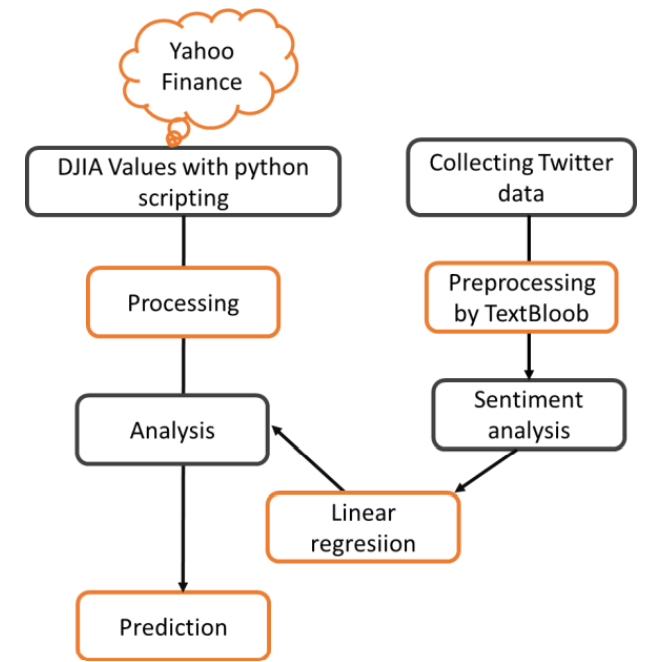
\includegraphics[scale=.7]{img3/diagram.png}
    \caption{System Model Block Diagram}
    \label{fig:Block Diagram}
\end{figure}


\section{Methodology}
While there was a lot of studies which was happened in classifying a bit of textual content as both positive or negative, there was little paintings on multi-magnificence classification. Sentiment analysis is a vital particle of our answer because this module of the output will be passed down for gaining knowledge of our predictive process. Natural language processing (NLP) is taken into consideration to be an effective device for expressing and decoding human languages like speech and textual content. Natural language processing is beneficial to textual content evaluation and textual content mining. In our experiment, we use Python and TextBlob library to perform a variety of sports related to sentiment analysis. As Python programming library has easy API, TextBlob is effortlessly able to acting primary NLP sports and tasks.\\


\section{System Design}
In this project, the system we want to evaluate the sentiment analysis tool which retrieves, processes and tests twitter data. The main purpose of our project to build a co-relation between stock prices and the overall people sentiment. At the very first step we have collected stock values from Yahoo Finance for a defined time range for our project. Next step, we have tried to collect the twitter trending data using twitter API at the same time range. Then we have pre- processed data we got from twitter and DJIA values. With textblob and python data-frame for featuring twitter data for analyzing sentiment. At the final step there is involved a linear regression algorithm for visualizing of data along with required tests.the full process is shown as a system architecture in figure 3.2. \\

\begin{figure}[h]
    \centering
    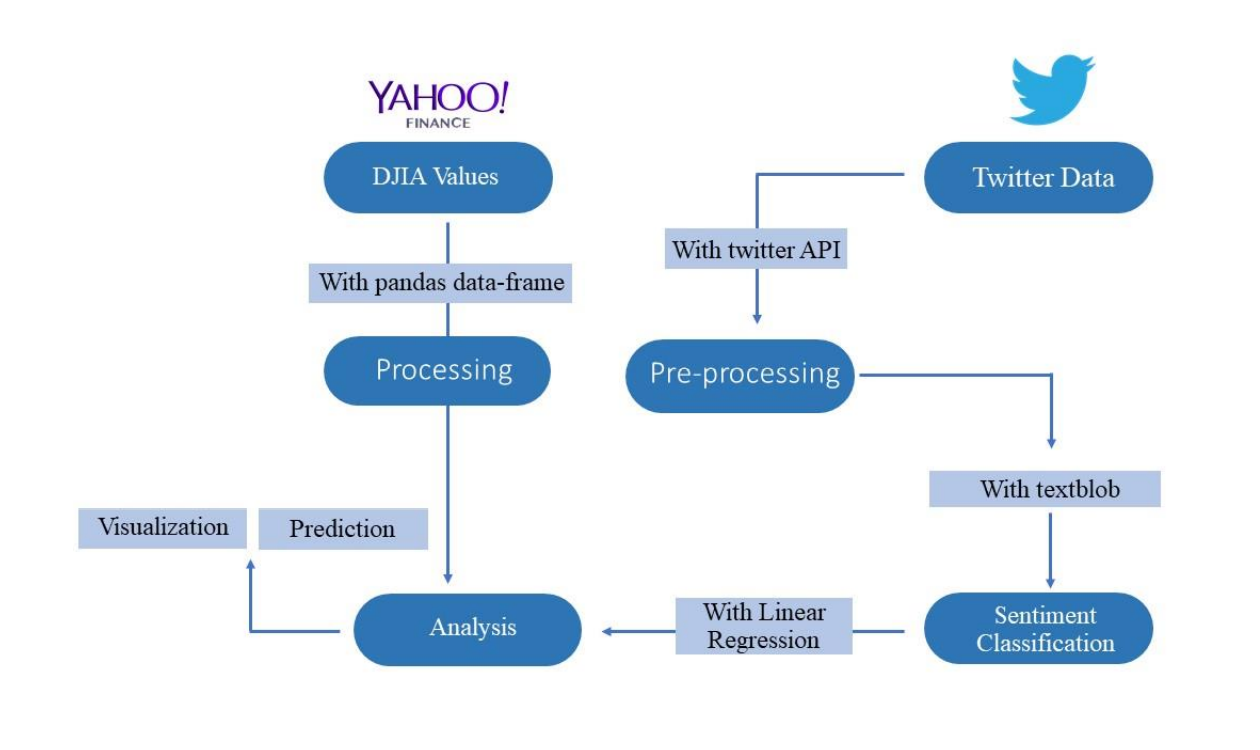
\includegraphics[scale=.6]{img3/System Architecture.png}
    \caption{System Architecture}
    \label{fig:System Architecture}
\end{figure}


\section{Data Set and Preprocessing}
Because the ways of data collection can get in large portions, it has become difficult to identify from which source we extract data or exactly which messages are selected for doing sentiment analysis. Raw inventory price statistics are pre-processed before inputting into machine getting to know various models. Pre-processing consists of reworking the uncooked records within a layout which process can take from and function on, most possibly characteristic matrix. It allows extracting some features, monetary-area-particular especially, manually to enhance outcomes, allowing the model to research greater abstractions. The data we have collected for this research is mainly from 2020 till now.\\

In our study, we’ve collected random twitter data by using Twitter API, which we applied for. For the need of our experiments, we’ve collected random Twitter posts of that point as numeric data. These numeric data associated with finances are collected from Yahoo! Finance website. The latter is that the property of Yahoo! was founded to supply economic and financial news and commentary covering share prices, financial press releases, financial reports, etc. We collect each data while aggregating numeric data supported attributes of share prices with opening, high, low and shutting rates (OHLC). This data set is critical because it is employed to support predictive analyses on the future movement of share prices.The dataset processing is illustrated in figure 3.3. \\


\begin{figure}[H]
    \centering
    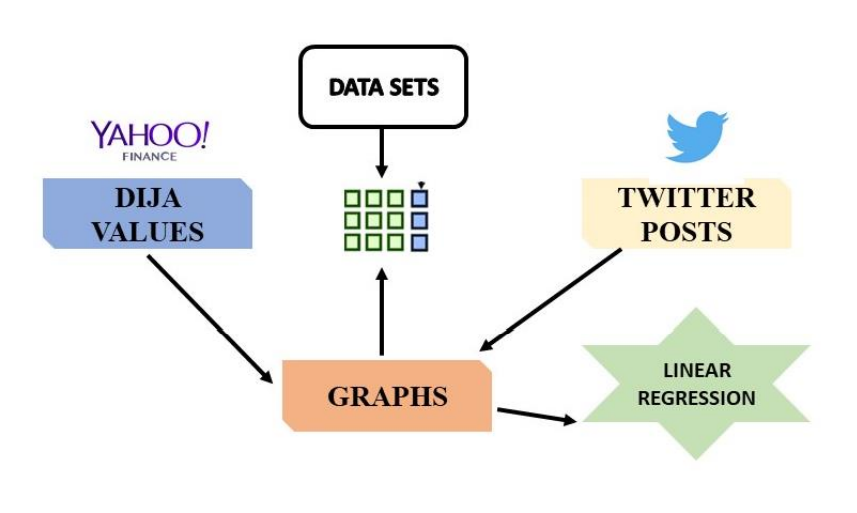
\includegraphics[scale=.65]{img3/Dataset Pre-processing.png}
    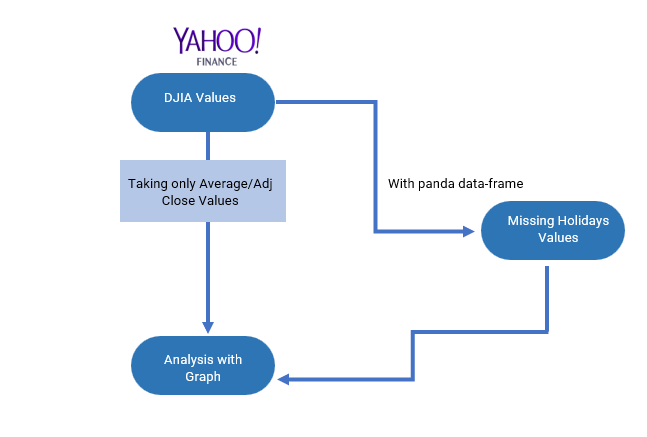
\includegraphics[scale=.9]{img3/Dataset Pre-processing2.png}
    \caption{Dataset Pre-processing}
    \label{fig:Dataset Pre-processing}
\end{figure}


\subsection{DJIA Value}

The main dataset for this study is the inventory stock data. For example, that index-wide variety industrial common (DJIA) is taken into consideration. 
To begin, create two variables: $start\_date$ and $end\_date$. If each date founds in yfinance, then the djia-values will be downloaded as a csv file, and finally the procedure has come to an end. Here, given below in the algorithm 1 which is used to extract DJIA data.\\

\begin{algorithm}
\caption{DJIA Data Extract}\label{alg:djia}
\begin{algorithmic}[1]
\State $each\_date \gets (start\_date, end\_date)$
\State $stock \gets 'dji'$
\For{$each\_date \in stock$}
    \If{$start\_date \leq end\_date$}
        \State $djia\_values \gets yfinance.download(stock,each\_date)$
    \EndIf
\EndFor
\State $djia\_data \gets pandas.dataframe(djia\_values)$
\\\textbf{Return}
\textit{djia\_data}
\end{algorithmic}
\end{algorithm}

The primary information for the stock price records became to be had on the Yahoo finance website. The know-how became accrued by writing a python script to carry out internet scraping.\\

\begin{figure}[H]
    \centering
    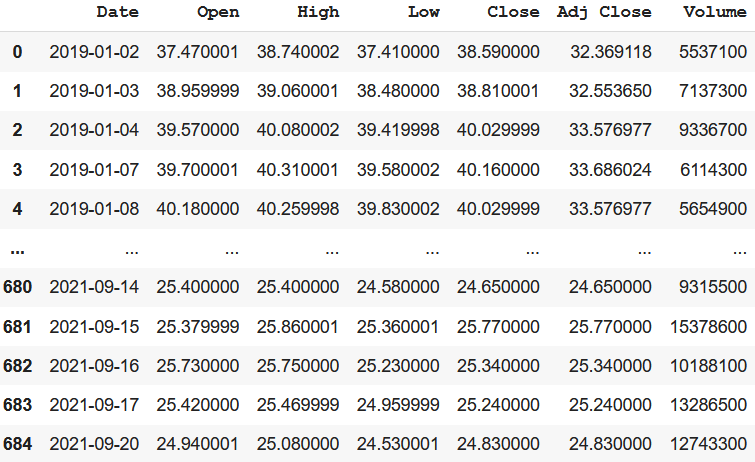
\includegraphics[scale=.8]{img3/Collected DJIA Values.png}
    \caption{Collected DJIA Values}
    \label{fig:DJIA Values}
\end{figure}

Through this net scraping shown in figure 3.4, the statistics are accumulated and stored as a comma-separated value (CSV) record. It’s to be cited right here that most effective the inter-day buying and selling values are acquired. This refers back to the trading performed across diverse days and intra-day refers to the trade carried out in the day. This can be because the intraday trading fees don’t appear to be readily available similar to the inter-day expenses and it also will increase the computational need and complexity. An additional piece of key statistics that may not be acquired is the order e-book. It can help provide a prediction of the rate using the weighted average of the orders.\\



\subsection{Twitter Data}
Tweets are on hand via a truthful seek of requisite phrases via a utility programming interface (API). Currently, over 500 million messages are published on Twitter on an everyday foundation as we can see in figure 3.5. This takes a look at turned into carried out over a length of eight months length that is already instructed in the introduction. During this era, we’re amassing English tweets wherein every tweet file contains various identifiers, languages, texts and different submitted dates/times to reach as we have directed our goal on trending tweets wherein tweets are different quite trades and mentioned generation stocks which have excessive tweet versions. \cite{bhardwaj2015sentiment}\\
\begin{figure}[H]
    \centering
    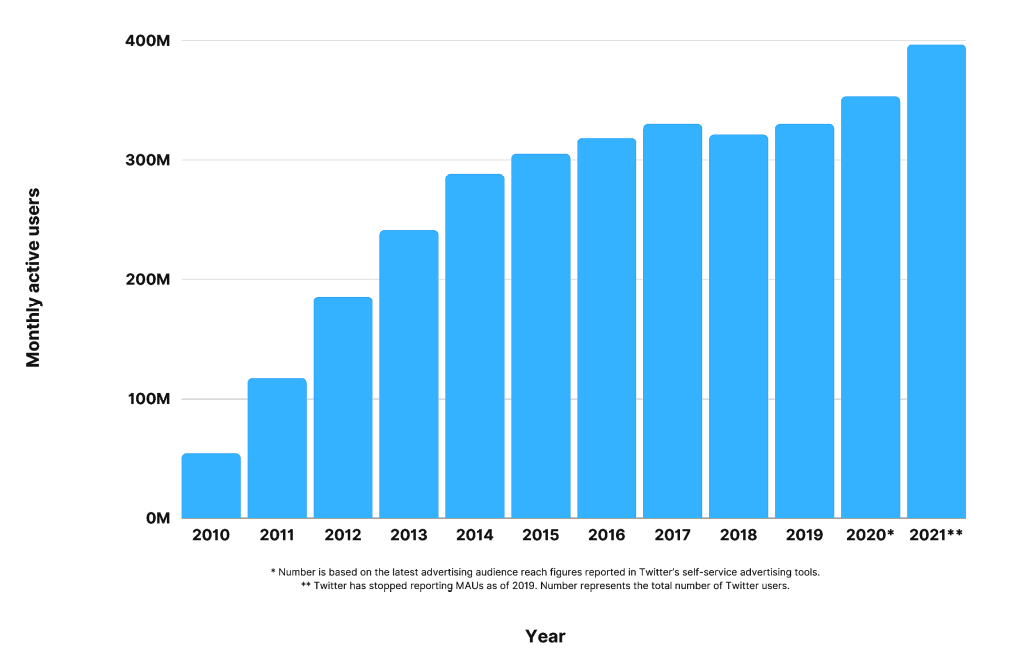
\includegraphics[scale=.5]{img3/Twitter Users.png}
    \caption{Twitter Users Growth}
    \label{fig:Twitter Users}
\end{figure}

While the Twitter statistics became to be had for all day mendacity withinside the given timeline, the DJIA values are required the usage of Yahoo! Finance website became missing data for weekends and different desertions while that marketplace is shut. To finish these statistics, we resembled those lacking ethics the usage of pandas data-frame work.\cite{noauthor_count_2020}\\

In the following steps how to obtain twitter API keys:
\begin{itemize}
    \item[--] Login to twitter developer section.
    \item[--] Go to “Create an App”.
    \item[--] Fill the details of the application.
    \item[--] Click on Create your Twitter Application
    \item[--] Details of your new app will be shown along with consumer key and consumer secret.
    \item[--] For access token, click” Create my access token”. The page will refresh and generate access token.
\end{itemize}
    
After getting twitter API, we try to collect and extract twitter data. In given below algorithm which is used to help collecting and extracting twitter data.\\

To extract data from Twitter, we'll need the API keys, which will allow us to start collecting data.We gained access to many keys after gaining access to the Twitter API.We use the following keys for data extraction: customer key, customer secret key, access key, access secret key, and access token key.We fixed these keys after initializing them as variables because they differed from user to user.We can get the author of any tweet using this API, which we use below with trending tweets available at different periods.Then, to get the available trending tweets on a specific day, we create a condition and put them into a try loop. If it doesn't work, we'll double-check the keys we received as well as our network connection.Then, in our trending data, we search for trending terms and select the most popular ones to create raw data, which we use to initialize for api search, q=word, and get the results of popular tweets.Finally, we save the tweet data as raw data for our collection using Pandas Frame.The algorithm 2 below, which is used to collect and extract Twitter data, is as follows:\\

\begin{algorithm}[H]
\caption{Twitter Data Extract and Collect}\label{alg:tweet}
\begin{algorithmic}[1]
\Require API Keys
\State $tweet\_data \gets variable to collect tweet data$
\State $consumer\_key \gets tweet api customer key$
\State $consumer\_secret \gets tweet api customer secrect key$
\State $access\_key \gets tweet api customer acess key$
\State $access\_secret \gets tweet api customer secret acess key$
\\\textbf{try}
    \State $\indent auth \gets tweepy.OAuthHandler(consumer\_key, consumer\_secret)$
    \State $\indent auth.set\_access\_token(access\_key, access\_secret)$
    \State $\indent api \gets tweepy.API(auth)$
    \State $\indent print('Authorized!')$
\\\textbf{except}
    \State $\indent print('Error!')$\\
    
\State $raw\_data \gets []$
\State $trending\_data \gets api.trends\_place(id=1)$
\For{$trending\_word \in trending\_data$}
    \For{$word \in trending\_word['trends']$}
        \State $raw\_data \gets tweepy.Cursor(api.search,q=word,type='popular')$
    \EndFor
\EndFor
\State $tweet\_data \gets pandas.dataframe(raw\_data)$
\\\textbf{Return}
\textit{tweet\_data}
\end{algorithmic}
\end{algorithm}


\section{Sentiment Analysis}
To categorize given contextual content in order to map it to elegance, sentiment analysis is used. Sentiment Analysis may be binary, i.e., high-quality or negative or multi-elegance with three or extra instructions involved. The sort of sentiment evaluation relies upon on dataset and reasoning method adopted. Researchers and stakeholders frequently diverge on their interpretation of courting that exists among sentiment evaluation and detection of emotion. While their factors of view may also fluctuate primarily based totally on their respective perspectives, researchers are united in adopting similar techniques. It is a manner to gauge or decide the emotion of the writer. The emotion can either be nice, bad or neutral. TextBlob’s sentiment characteristic evaluates to 2 properties polarity and subjectivity. Subjectivity belongings values also are flow that falls inside the variety of [0, 1]. How we have worked on our project with text blob are shown in the following figure 3.6:\\

\begin{figure}[H]
    \centering
    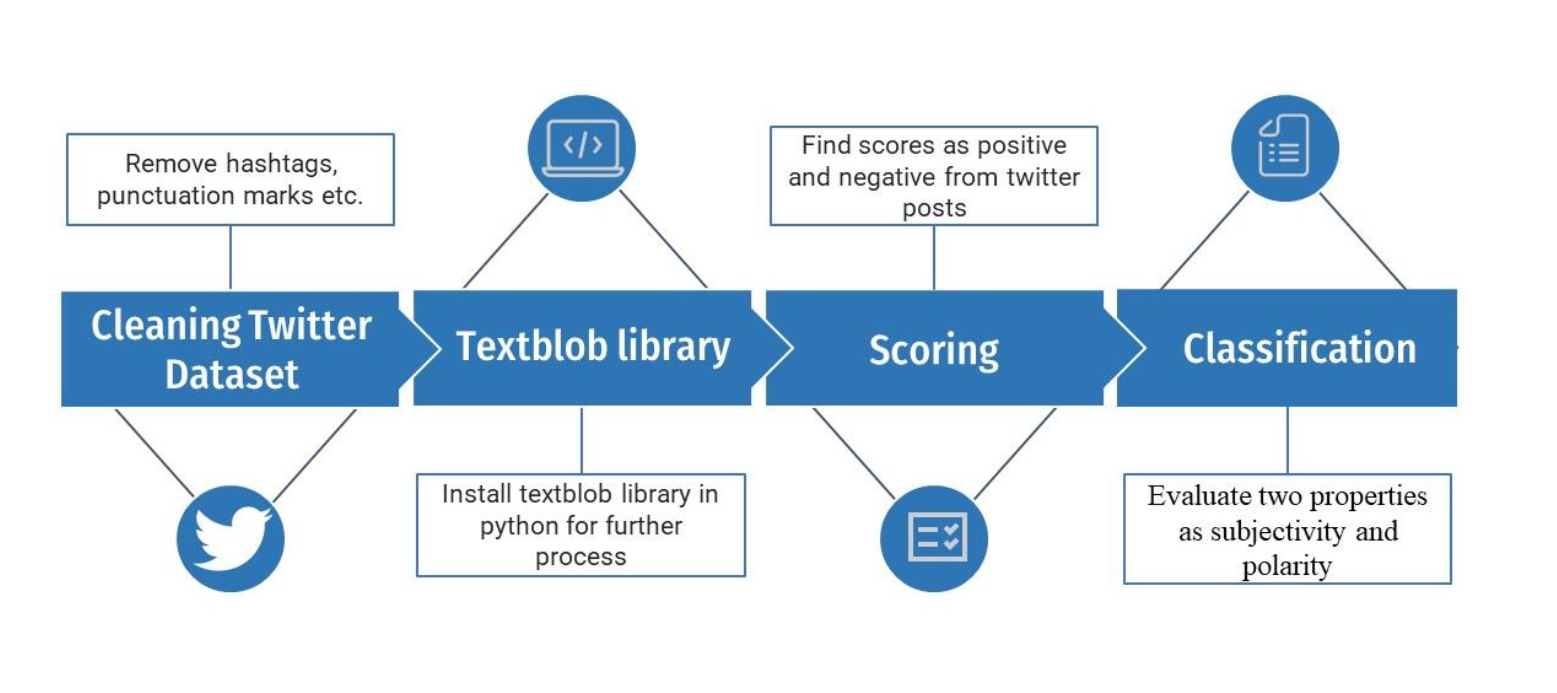
\includegraphics[scale=.45]{img3/Textblob Working Process.png}
    \caption{Textblob Working Process}
    \label{fig:Textblob}
\end{figure}

n this study, the opinion of various peoples of various countries has been discussed. the most focus of this paper is on Twitter, Twitter API and have implemented the python artificial language and to implement the sentimental analysis as positive, negative and neutral. 
In order to make the Twitter API more relevant, we'll first import Tweepy. Then use tweet data, all tweets, tweet value, SE (set of emoji), SSC (set of special characters), SP (set of punctuations), and clean tweet as variables. Following that, we'll download tweets as datasets and save them to a CSV file. Additionally, the all-tweets variable is used to get tweets from the dataset, and the SE, SSC, and SP variables are used to remove and eliminate harmful emoji, \#tags, special characters, and punctuation from tweets. Create a new CSV file for all clean tweets. The given algorithm helps us to organize and sanitize Twitter data. \\

\begin{algorithm}
\caption{Tweet Filtering Algorithm}\label{alg:Filter}
\begin{algorithmic}[1]
\Require $tweet\_data$
\State $temoji \gets set of Emojis$
\State $schar \gets set of special characters$
\State $punc \gets set of punctuations$
\\
\State $raw\_tweets \gets tweet\_data$
\For{$tweet \in raw\_tweet$}
    \If{$emoji = schar = punc \not= [NULL]$}
        \State $clean\_tweet \gets remove \in emoji, schar, punc$
    \EndIf
\EndFor
\State $clean\_data \gets pandas.dataframe(clean\_tweet)$
\\\textbf{Return}
\textit{clean\_data}
\end{algorithmic}
\end{algorithm}



We’ll tokenize every phrase withinside the dataset and keep it into the dataset. for each phrase, will evaluate it with positive, terrible and impartial sentiments phrase withinside the dictionary. Then increment the positive, terrible and impartial count. Finally, based totally on the positive, terrible and impartial count, we are ready to get the top result percent approximately sentiment to see the polarity. this study suggests the sentimental evaluation set of rules at an excessive level. As may be visible withinside the algorithm 3, researchers have distinct approaches to attach the Twitter API, four fetch the tweets, tweet cleansing or do away with preventing phrases and punctuation marks, classify tweets because of this that get the polarity of the tweet, and finally go back the results. In this paper, python is used to put in force the sentimental evaluation. Some applications have been applied along with tweepy and textblob.[6] \cite{mittal2012stock} The required 
libraries are mounted with the aid of using following commands:\\
$\blacktriangleright$ pip set up tweepy\\$\blacktriangleright$ pip set up textblob\\

The main steps of this sentiment analysis are drawn in following figure 3.7:\\

\begin{figure}[H]
    \centering
    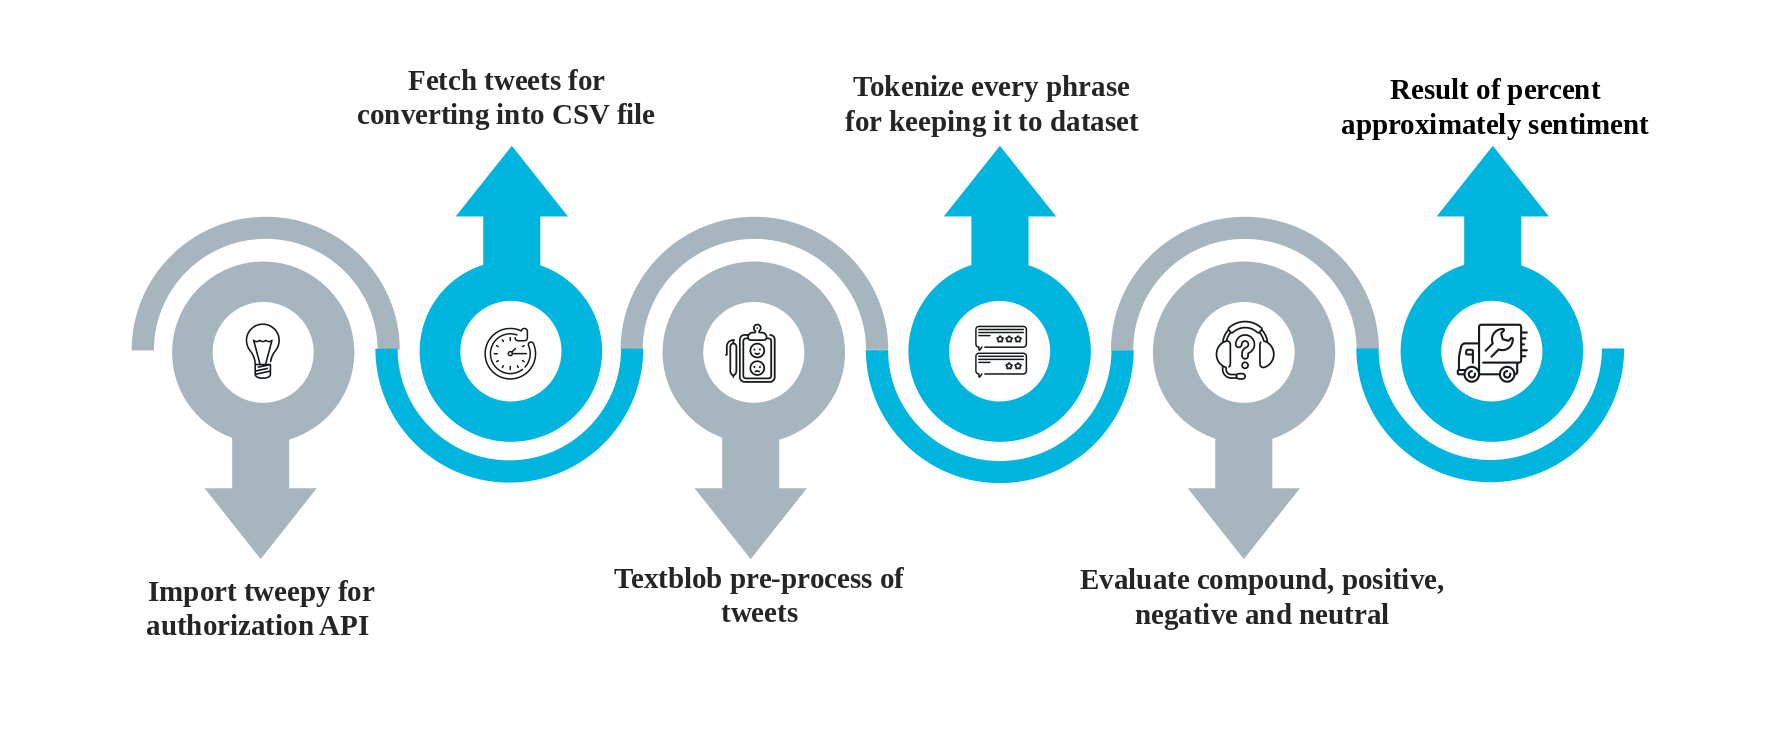
\includegraphics[scale=.3]{img3/Sentiment Analysis Process.png}
    \caption{Sentiment Analysis Process}
    \label{fig:Sentiment Analysis}
\end{figure}


\section{Hypothesis and Final Co-relation}
For getting better result and prediction, we at first find out the p-value of our twitter data. We applied this co-efficient so that we can know whether the prediction of our data will be possible to get or not. A probability associated with a crucial value is known as a p-value. The crucial value is determined by the possibility of a Type mistake being allowed. It calculates the probability of achieving results that are as least as good as if the claim (H0) were true.\\

A correlation matrix is a table that displays the coefficients of correlation between variables. The correlation between two variables is shown in each cell of the table. A correlation matrix can be used to summarize data, as an input to a more sophisticated study, or as a diagnostic tool for advanced analyses.The instances in a predicted class are represented by the rows of the matrix, whereas the instances in an actual class are represented by the columns (or vice versa). The name is derived from the fact that it is simple to observe if the system is mixing up two classes (i.e. commonly mislabeling one as another). It's a unique type of contingency table with two dimensions ("polarity" and "subjectivity") with identical sets of "classes" in each dimension. As we know if p-value is stayed at between 0 to 0.1 it is possible to make prediction on that dataset. After applying p-value we got the average result 0.06, 0,07 and 0.3. We know the range of p value is -1 to 1. Since our result is 0.06,0.07,0.3 so, ours dataset is ready for working . The p-value correlation coefficient of our dataset is given below in figure 3.8: \\

\begin{figure}[H]
    \centering
    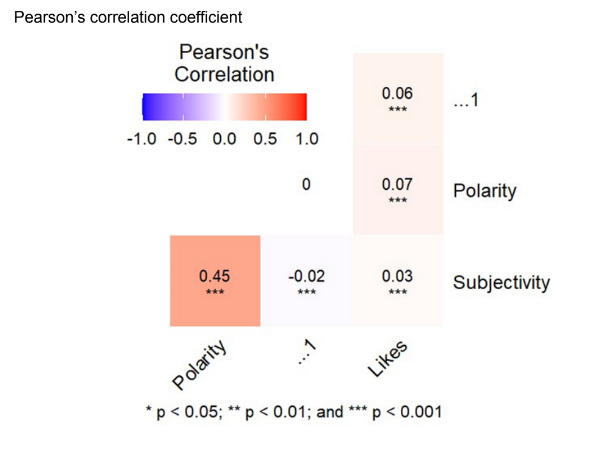
\includegraphics[scale=.9]{img3/Pearson.png}
    \caption{Pearson’s correlation coefficient}
    \label{fig:Pearson’s correlation coefficient}
\end{figure}

This study will try to show the following hypothesis in order to analyze the market.\\
H1: The total averaged sentiment of all stocks within a sector will be used to determine the
sentiment of the sector.\\
By using people sentiment, we will be able to identify their positive, negative thinking and whether their thinking is affecting a particular sector or not. The result of this hypothesis is clearly shown and explained in our result section with appropriate values and graph.\\\\
H2: On any given day, the sentiment of a sector or stock will provide a forecast for that stock’s
movement the next day.\\
We will know if the stock price will be up or down the next day or next moment of any day. By using this hypothesis, it will be easier for making any decisions to invest at their will. The overall prediction and accuracy level have been compared with our predicted values. To understand better it has been explained in detail at the result section with scatter plot by applying linear regression on our data.\\\\
H3: The stocks with the highest number of Twitter mentions are also the stocks that lend the
most weight to a sector’s mood.\\
From this thinking, we can know which type of sentiments are actually making effect on stock prices. The sentiments of tweet will be clearly shown with related graph and values to understand. We will work on more data so that we can understand people’s mood who are directly investing on share market. To know their mood, we need more data and also need to do real time survey on those people which will be time consuming so far for which we will work in future on that.\\

\section{Linear Regression (Proposed Algorithm)}
The linear regression set of rules tries to research a characteristic that maps enter vectors to scores. It represents with the aid of using a linear mixture of the enter capabilities. We will try to use an ahead step-clever technique to set the mass in order to carry out the characteristic collection. At the very early stage, we have to fix the implied evaluation rating. After this, till the favored variety of entering capabilities were delivered, enter capabilities have been delivered differentially. At every stride, that characteristic which will minimize corrupted mistakes maximum when delivered became collected. If the time of delivering, its mass fixes as if corrupted mistakes could be reduced, then given that capabilities and mass already delivered. That variety to enter capabilities consisting of became decided with the aid of using validation \cite{bhardwaj2015sentiment}. The working process of this algorithm is drawn at step by step in the following figure 3.9:
\begin{figure}[H]
    \centering
    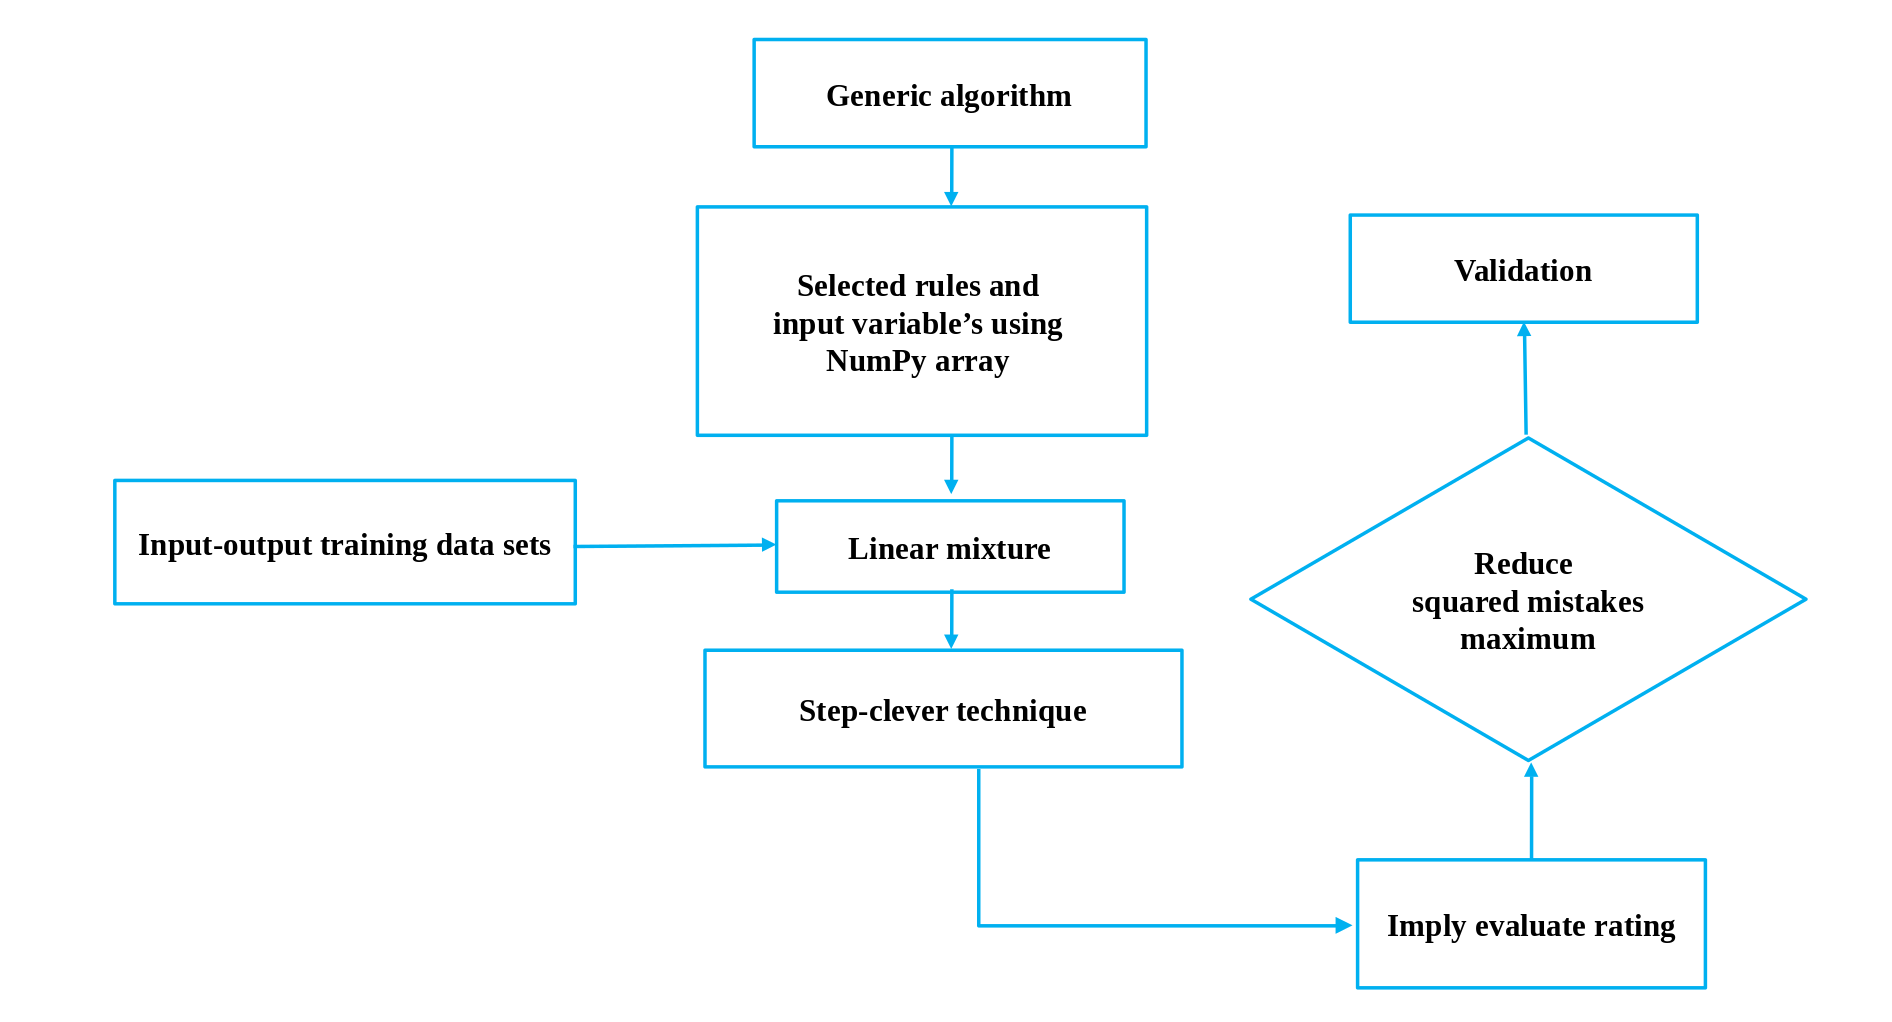
\includegraphics[scale=.3]{img3/Linear Regression Workflow.png}
    \caption{Linear Regression Workflow}
    \label{fig:LR Workflow}
\end{figure}

 
 \label{chap3:Result and Analysis}
 \input{chapters/chapter4}

 
 \label{chap3:Conclusion}
 \chapter{Conclusion and Future scope}
Using data from Yahoo Finance, this research constructs a model and algorithm for stock price prediction. Traders, investors, and analysts benefit from efficient and accurate stock price prediction systems since they provide helpful information such as the stock market's future direction. For the best accuracy, we discovered that historical data should be used for Linear Regression. Data scientists' possibilities for solving fascinating problems with high accuracy are expanding thanks to deep learning technologies. We used a large scale collection of tweet data to uncover links between Twitter-based sentiment analysis of a particular company/index and its market performance in this article. Our findings reveal that negative and positive aspects of public mood have a strong cause-and-effect relationship with individual stock/index price changes. We also looked into how prior week sentiment features influence the opening and closing values of stock indexes for various tech businesses and important indexes such as the DJIA and NASDAQ-100.Our findings are in some ways similar, but there are some significant variances. To begin, our findings reveal a stronger association between negative and positive mood dimensions and DJIA values, as opposed to their findings, which showed a strong correlation with only the good mood dimension. Second, while we were unable to achieve a high percentage result of 87 percent, our 73 percent result using Linear regression provides better proof that the connection exists over the full data set.\\



Finally, numerous factors are left out of our analysis. To begin with, our dataset does not represent true public mood; it only takes into account persons who use Twitter and speak English. When the actual mood is analyzed, it is feasible to establish a higher correlation. The association could be explained by the fact that people's moods influence their financial decisions. However, there is no clear link between persons who invest in stocks and those who use Twitter more regularly, however there is an indirect link: people's investment decisions may be influenced by the emotions of those around them, i.e. general public attitude. All of these will continue to be investigated in the future.\\

\label{chap4:Reference}
\bibliographystyle{ieeetr}
% \renewcommand{\bibname}{Bibliography}
\bibliography{ref.bib}

\end{document}
